
%%% Local Variables:
%%% mode: latex
%%% TeX-master: t
%%% End:

\chapter{引言}
\label{cha:intro}
\section{研究背景}
\subsection{Web Service}
随着20世纪90年代互联网技术的快速发展以及电子商务大规模部署,企业级软件也从大规模集中的复杂软件向分布式松耦合的Web服务进化。SOA(service-oriented architecture, 面向服务体系架构)作为一种新的软件设计概念被提出来。虽然没有对SOA统一的确定性定义,但普遍指一种基于开放的协议或标准,将松耦合、自治的功能服务进行整合的设计思想。而随着面向服务的网络服务设计思想的普及,一些企业联盟及组织也制订了Web服务的通用标准与协议。W3C组织将Web服务(Web Service)定义为支持通过网络机器之间互操作的软件系统。\cite{haas2004web}同时工业界逐渐接收基于SOAP(Simple Object Access Protocol)协议的Web Service架构。
\subsubsection{SOAP服务架构概述}
SOAP协议指简易对象访问协议。在Web Service架构中作为格式化信息交换协议。SOAP协议定义类以XML格式为基础的数据封装格式,定义了数据格式,远程调用与应答的封装。SOAP协议虽然不限制下层的通信协议,但是普遍采用HTTP协议与当前浏览器兼容。以SOAP协议为基础,Web Service的三大组件分别为SOAP,WSDL(Web Services Description Language,网络服务描述语言)及UDDI(Universal Description Discovery and Integration,统一描述、发现和集成协议)。WSDL是基于XML用来描述Web Service服务的文档语言。通过WSDL文档以规定Web Service所执行的操作,使用的消息,数据类型以及需要绑定的通信协议。UDDI提供了一种Web Service的目录服务,提供了一种通过Internet来注册Web Service信息,来促进Web Service互相发现与利用的检索与集成服务。

一个典型的Web Service如图\ref{fig:web-service-arc}所示。服务请求者和服务提供者通过SOAP协议进行通信。而服务提供者将服务描述注册到服务协调者UDDI上。服务请求者可以通过服务协调者获得该服务的操作接口,也可以对多个服务进行服务组合。
\begin{figure}[H]
  \centering
  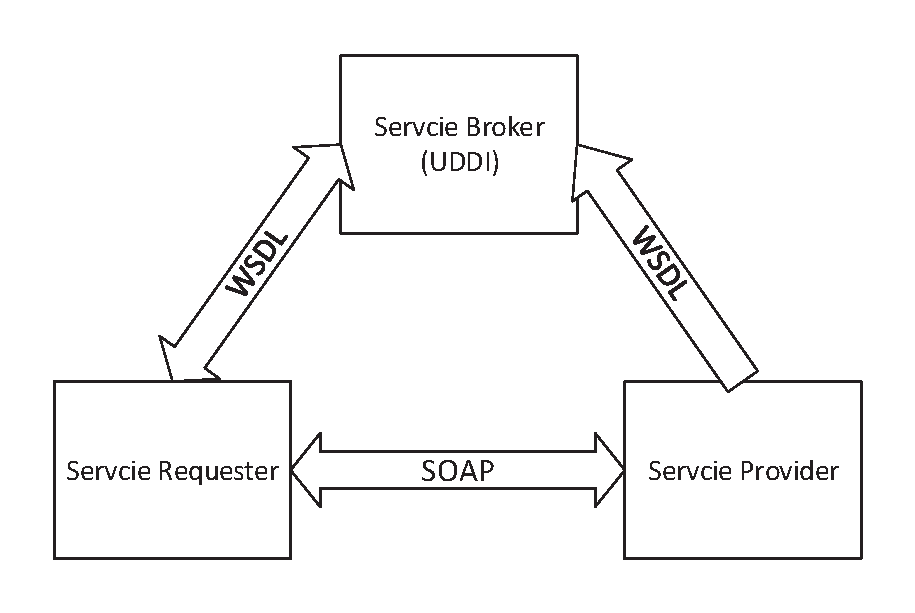
\includegraphics[width=0.6\textwidth]{web-service-arc}
  \caption{Web Service典型架构}
  \label{fig:web-service-arc}
\end{figure}

\subsubsection{REST服务架构概述}
REST(Representational state transfer)并不是特指具体一种通信协议,而是一种扩展服务设计的原则。随着近些年云服务的开展普及,REST在工业界得到了非常广泛的应用,如Amazon S3,微信公共账号接口等。与SOAP协议不同,REST需要直接利用HTTP协议作为传输协议,利用HTTP动词(GET,POST,PUT,DELETE)与URI的组合来定义REST的具体服务操作。

\subsubsection{存在的问题}

对于当前最普遍的两种Web服务架构即基于SOAP与REST普遍是现在HTTP协议之上。在SOAP中,包含服务请求与应答的XML报文直接封装在HTTP数据包之中。在REST中,资源直接通过HTTP的URI进行标记,通过HTTP动词对资源进行操作。HTTP协议已经成为事实上的网络瘦腰(narrw waist)。\cite{popa2010http}但以HTTP为承载的服务网络包含如下问题:HTTP为应用层协议,到物理层信号传输还要经过多层次的协议栈。而相关的经典协议栈如IP协议、以太网协议等兼顾通用性,未对事实上的瘦腰HTTP协议进行优化。例如HTTP协议无法阻止在底层网络层面阻止DDOS攻击,网络层面无法直接缓存数据包,需要服务提供商自建或租用CDN系统。REST架构的网络服务中,本质是面向资源,面向内容的状态控制变化的,客户端不需要关心服务或资源的具体位置。而当前底层最普遍的IP网络是面向连接的,在处理相同资源在不同的物理地址路由时,无法做到面向内容的优化路由。

\subsection{信息中心网络概述}

随着当今互联网数据分发流量的快速增长,TCP/IP架构在内容分发方面暴露出一些问题。因此信息中心网络(Information Centric Networking,ICN)作为一种新的网络架构设计原则被提出来。目前正在积极研究并开发的ICN网络项目有:DONA(Data-Oriented Network Architecture)\cite{koponen2007data},Named Data Networking(NDN)\cite{jacobson2009networking},Content-Centric Networking(CCN)\cite{jacobson2009networking},Publish-Subscribe Internet Routing Paradigm(PRISP)\cite{ain2009d2},Network of Information(NetInf)\cite{ahlgren2010second}等。虽然实现方式细节上各有不同,但是设计目标与架构特点相似。都是为了更有效率地获取与分发数据,并解决网络中断,流量洪泛等问题。网络通信通常由数据请求端驱动。网络包单位为命名数据对象(named data object,NDO)。\cite{ahlgren2012survey}ICN对于传统的TCP/IP架构网络的颠覆则是利用NDO来替代IP包作为新的网络瘦腰。

\section{研究内容及意义}
本论文主要研究利用信息中心网络的命名数据机制设计一种新的面向服务的网络架构,并对该架构进行原型实现与实验评估。具体研究内容为:
\begin{itemize}
\item 提出一种基于命名机制的服务网络协议设计,即命名服务网络协议;
\item 以命名服务网络协议为基础设计一套服务网络架构,包括服务发现,服务路由,安全验证,服务仲裁等组件
\item 提出一套服务网络比较框架,并与SOAP与REST的网络服务架构进行比较分析
\item 根据命名服务网络架构设计一种本地分布式计算系统方案
\end{itemize}
研究意义在于打破传统服务网络基于HTTP协议与TCP/IP面向连接的网络架构,充分利用信息中心网络的性质特点提出一种新的网络设计范式,并未未来服务网络实现提供一种可能方案。
\section{章节安排}
本论文公分7章,各章内容如下:

第一章介绍课题的背景与研究意义。

第二章介绍本文涉及到的服务网络包括Web Service以及信息中心网络的基本概况与研究进展。重点介绍命名数据网络的架构以及当前的开发动态。同时多种介绍基于信息中心网络的服务架构研究,分析比较各个研究特点并总结不足。

第三章介绍作者参与的基于命名数据网络存储软件的开发细节,并总结出基于命名数据网络服务开发的原则。

第四章介绍命名服务网络的协议与架构设计。

第五章进行命名服务网络的原型实现,并基于该原型进行实验评估。

第六章提出一种基于命名服务网络的本地分布式服务集群设计

第七章对前面所做工作进行总结并指出未来需要完善的工作,并对未来研究做出展望。

